\subsection{ทดสอบประสิทธิ์ภาพการทำงานของโมเดลปัญญาประดิษฐ์สำหรับการระบุตัวตนของบุคคล}
ความแม่นยำของโมเดลปัญญาประดิษฐ์จากแหล่งที่มีมามีค่าดังตารางด้านล่างดังนี้
\begin{table}[!ht]
\centering
\begin{tabular}{|c|c|}
		\hline
		{โมเดลปัญญาประดิษฐ์}&{rank1/mAP โดยใช้วิธีการทดสอบด้วย Global+DMLI}				\\
		\hline
		ResNet50 Market1501	 			& 91.0/77.6								\\
		ResNet50 DukeMTMCReID			& 80.7/68.0								\\
		ResNet50 CUHK03				& 60.9/59.7								\\
		ResNet50 MSMT17				& 66.3/40.6								\\
	\hline
\end{tabular}
\caption{ผลการทดสอบความแม่นยำของโมเดลปัญญาประดิษฐ์}
\label{tab: Accuracy of model ReID}
\end{table}
ต่อมานำโมเดลปัญญาประดิษฐ์แต่ละอันมาทดสอบกับตัวอย่างภาพชุดข้อมูลที่ทางคณะผู้วิจัยได้สร้างขึ้น โดยภาพชุดข้อมูลที่นำมาใช้จะผ่านการตรวจหาบุคคลภายในภาพด้วยโมเดลปัญญาประดิษฐ์ YoLo v3 320
\begin{figure}[!ht]
    \centering
    \begin{subfigure}[b]{0.2\textwidth}
        \centering
        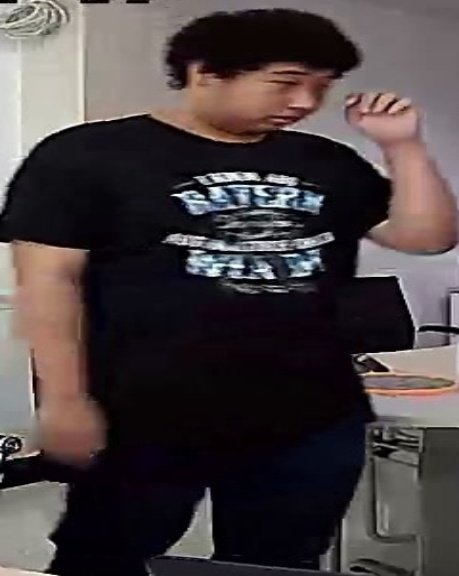
\includegraphics[width=\textwidth]{chapter4/images/o_0.jpg}
        \label{fig:ex_1}
    \end{subfigure}
    \begin{subfigure}[b]{0.2\textwidth}
        \centering
        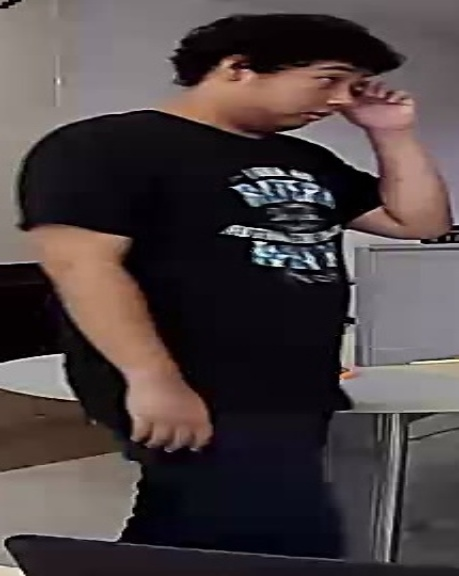
\includegraphics[width=\textwidth]{chapter4/images/o_1.jpg}
        \label{fig:ex_2}
    \end{subfigure}
    \caption{ภาพตัวอย่างชุดข้อมูลสำหรับการทดลองครั้งที่ 1}
    \label{fig: ภาพตัวอย่างชุดข้อมูลสำหรับการทดลอง 1}
\end{figure}
\begin{table}[!ht]
\centering
\begin{tabular}{|c|c|}
		\hline
		{โมเดลปัญญาประดิษฐ์}&{ค่าสำหรับการระบุบุคคล (Original distance)}							\\
		\hline
		ResNet50 Market1501	 			& 0.4308								\\
		ResNet50 DukeMTMCReID			& 0.4827								\\
		ResNet50 CUHK03				& 0.4914								\\
		ResNet50 MSMT17				& 0.4668								\\
	\hline
\end{tabular}
\caption{ผลการทดสอบความแม่นยำสำหรับการระบุบุคคลของโมเดลปัญญาประดิษฐ์ครั้งที่ 1}
\label{tab: Original distant of image 1}
\end{table}
\begin{figure}[!ht]
    \centering
    \begin{subfigure}[b]{0.2\textwidth}
        \centering
        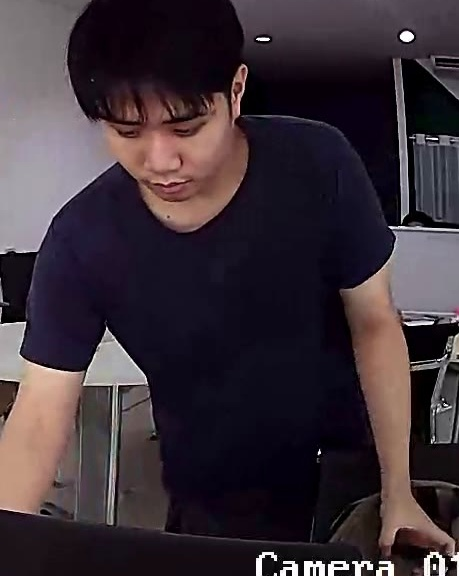
\includegraphics[width=\textwidth]{chapter4/images/first_0.jpg}
        \label{fig:ex_3}
    \end{subfigure}
    \begin{subfigure}[b]{0.2\textwidth}
        \centering
        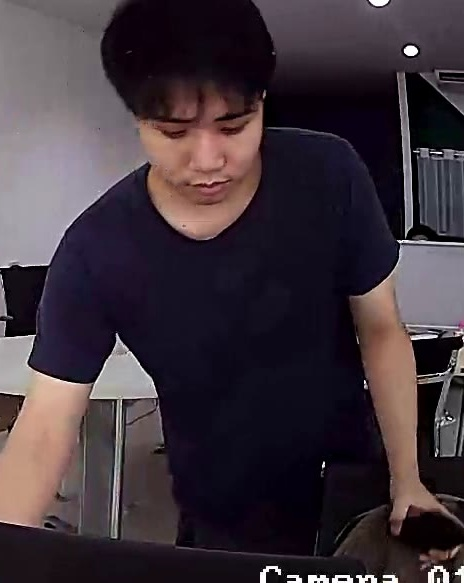
\includegraphics[width=\textwidth]{chapter4/images/first_1.jpg}
        \label{fig:ex_4}
    \end{subfigure}
    \caption{ภาพตัวอย่างชุดข้อมูลสำหรับการทดลองครั้งที่ 2}
    \label{fig: ภาพตัวอย่างชุดข้อมูลสำหรับการทดลอง 2}
\end{figure}
\begin{table}[!ht]
\centering
\begin{tabular}{|c|c|}
		\hline
		{โมเดลปัญญาประดิษฐ์}&{ค่าสำหรับการระบุบุคคล (Original distance)}							\\
		\hline
		ResNet50 Market1501	 			& 0.3035								\\
		ResNet50 DukeMTMCReID			& 0.3332								\\
		ResNet50 CUHK03				& 0.3	042								\\
		ResNet50 MSMT17				& 0.3684								\\
	\hline
\end{tabular}
\caption{ผลการทดสอบความแม่นยำสำหรับการระบุบุคคลของโมเดลปัญญาประดิษฐ์ครั้งที่ 2}
\label{tab: Original distant of image 2}
\end{table}
\clearpage
\begin{figure}[!ht]
    \centering
    \begin{subfigure}[b]{0.2\textwidth}
        \centering
        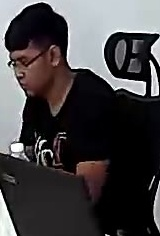
\includegraphics[width=\textwidth]{chapter4/images/fei_0.jpg}
        \label{fig:ex_5}
    \end{subfigure}
    \begin{subfigure}[b]{0.2\textwidth}
        \centering
        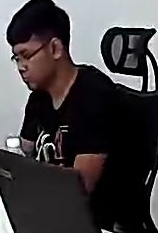
\includegraphics[width=\textwidth]{chapter4/images/fei_1.jpg}
        \label{fig:ex_6}
    \end{subfigure}
    \caption{ภาพตัวอย่างชุดข้อมูลสำหรับการทดลองครั้งที่ 3}
    \label{fig: ภาพตัวอย่างชุดข้อมูลสำหรับการทดลอง 3}
\end{figure}
\begin{table}[!ht]
\centering
\begin{tabular}{|c|c|}
		\hline
		{โมเดลปัญญาประดิษฐ์}&{ค่าสำหรับการระบุบุคคล (Original distance)}							\\
		\hline
		ResNet50 Market1501	 			& 0.3308								\\
		ResNet50 DukeMTMCReID			& 0.3296								\\
		ResNet50 CUHK03				& 0.3	134								\\
		ResNet50 MSMT17				& 0.3968								\\
	\hline
\end{tabular}
\caption{ผลการทดสอบความแม่นยำสำหรับการระบุบุคคลของโมเดลปัญญาประดิษฐ์ครั้งที่ 3}
\label{tab: Original distant of image 3}
\end{table}
ค่าความแม่นยำในการระบุบุคคลนั้นค่ายิ่งเข้าใกล้ 0 แสดงบุคคลใน 2 เฟรมนั้นเป็นบุคคลเดียวกัน จากการทดลองครั้งที่ 1 จะเป็นเฟรมที่ไม่ต่อเนื่องกัน การทดลองครั้งที่ 2 และ 3 นั้นจะเป็นเฟรมที่ต่อเนื่องกันมากขึ้นตามลำดับ ซึ่งจะแสดงให้เห็นว่าโมเดลปัญญาประดิษฐ์ที่สามารถให้ผลลัพท์ที่มีประสิทธิภาพต่อเนื่องมากที่สุดคือ ResNet50 Market1501
